\setauthor{Isabel Schnalzenberger}

\section{Technologien}

\subsection{Unity}

Unity ist eine leistungsstarke Laufzeit- und Entwicklungsumgebung (IDE) für Spiele, auch als Spiel-Engine (bzw. Gameengine) bekannt, die von Unity Technologies mit Hauptsitz in San Francisco entwickelt wurde. Diese vielseitige Plattform ermöglicht die Erstellung von Spielen und interaktiven 3D-Grafik-Anwendungen für verschiedene Zielplattformen, darunter PCs (Windows und Mac), Spielkonsolen, mobile Geräte und Webbrowser.\footnote{Alle Infos zu Unity stammen von: \cite{UnityDocs}}

\begin{figure} [h t]
    \centering
    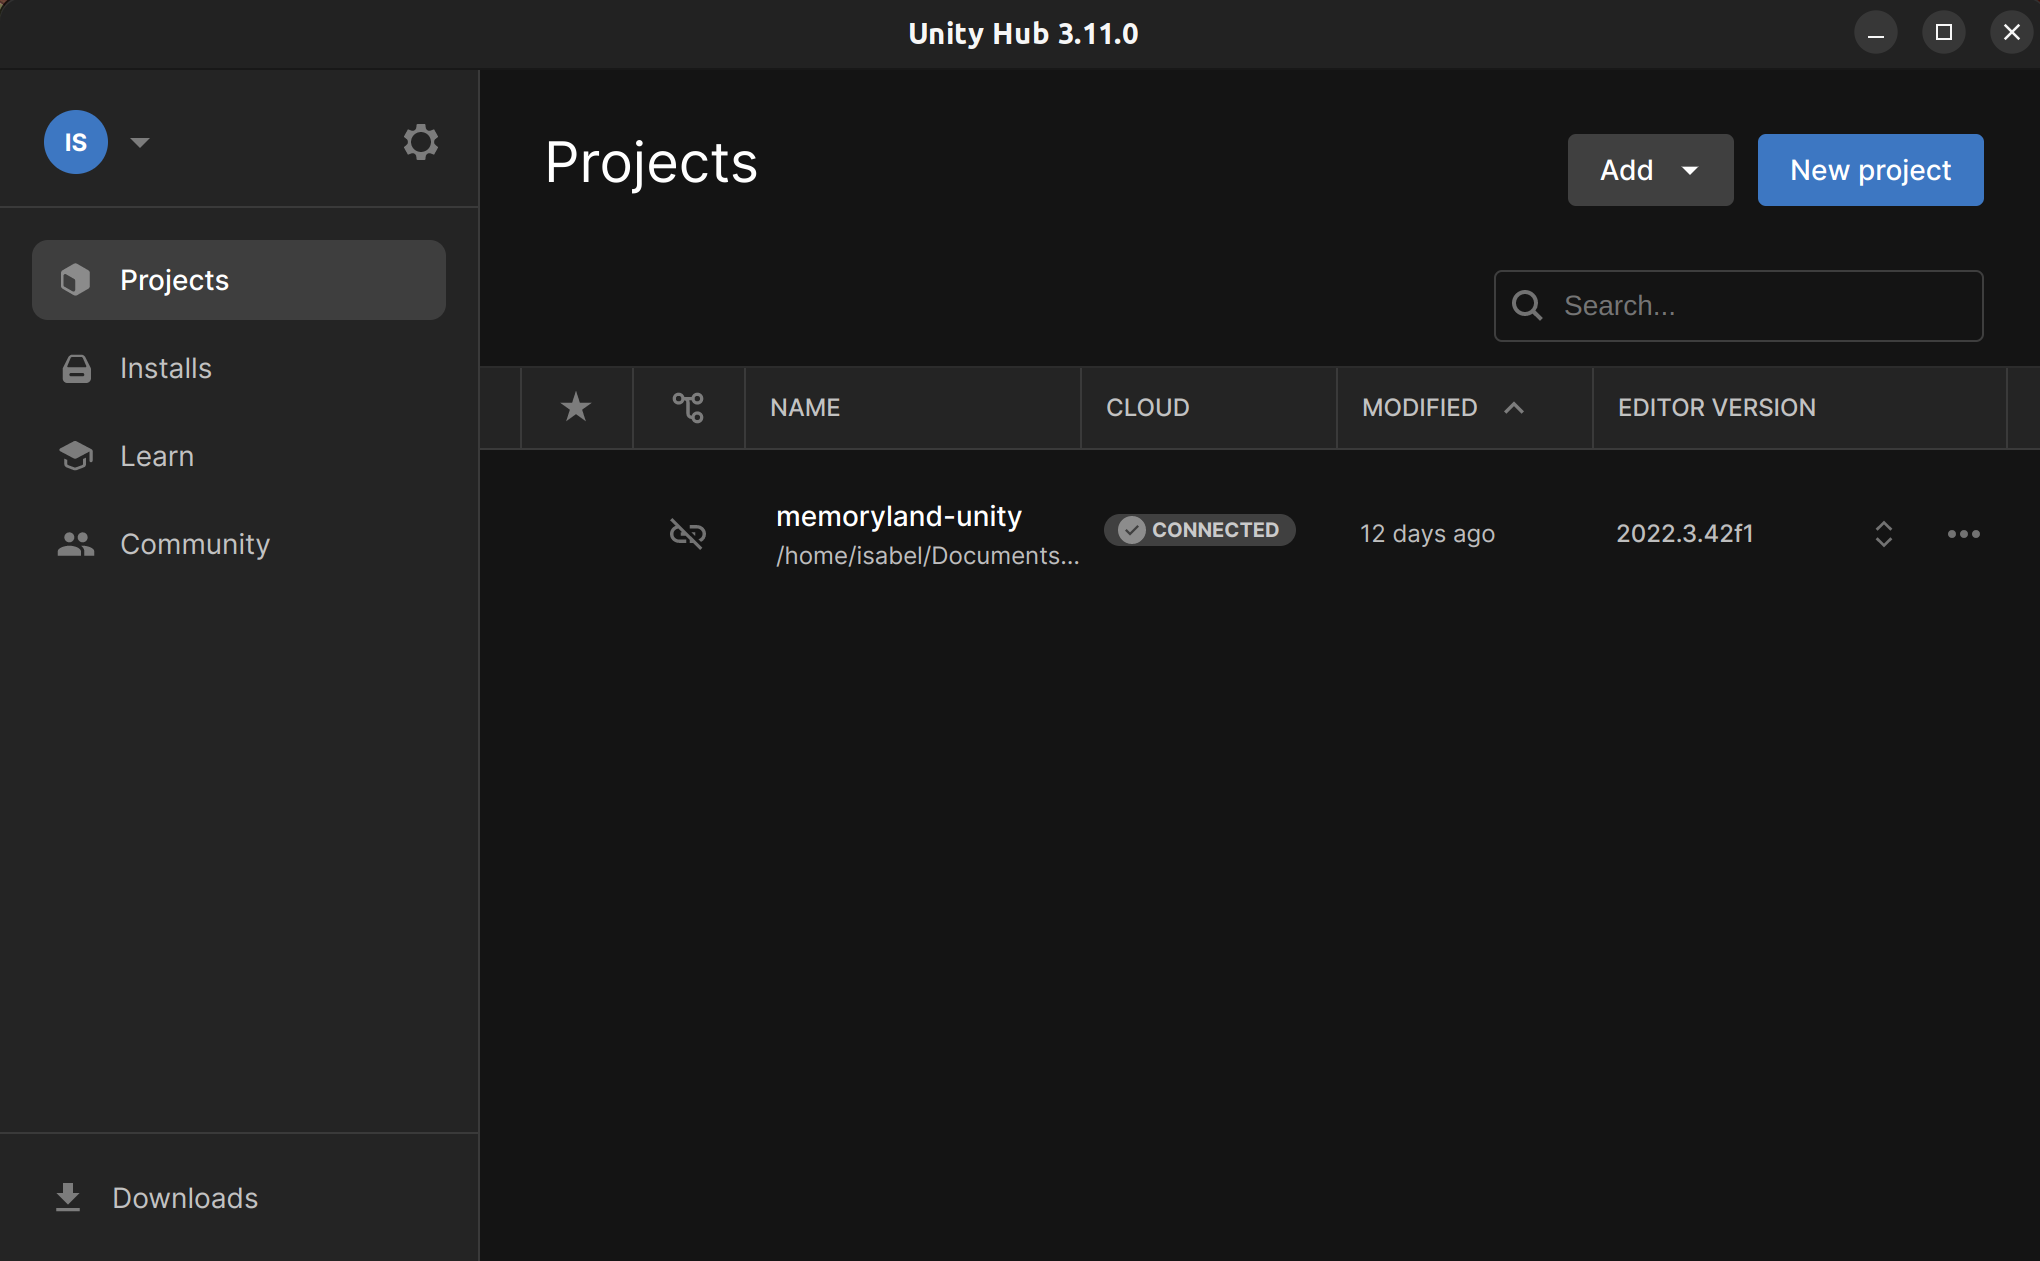
\includegraphics[scale=0.5]{pics/unity-hub.png}
    \caption{Entwicklung in Unity: der Unity-Hub}
    \label{fig:unity-hub}
\end{figure}


\begin{figure} [h t]
    \centering
    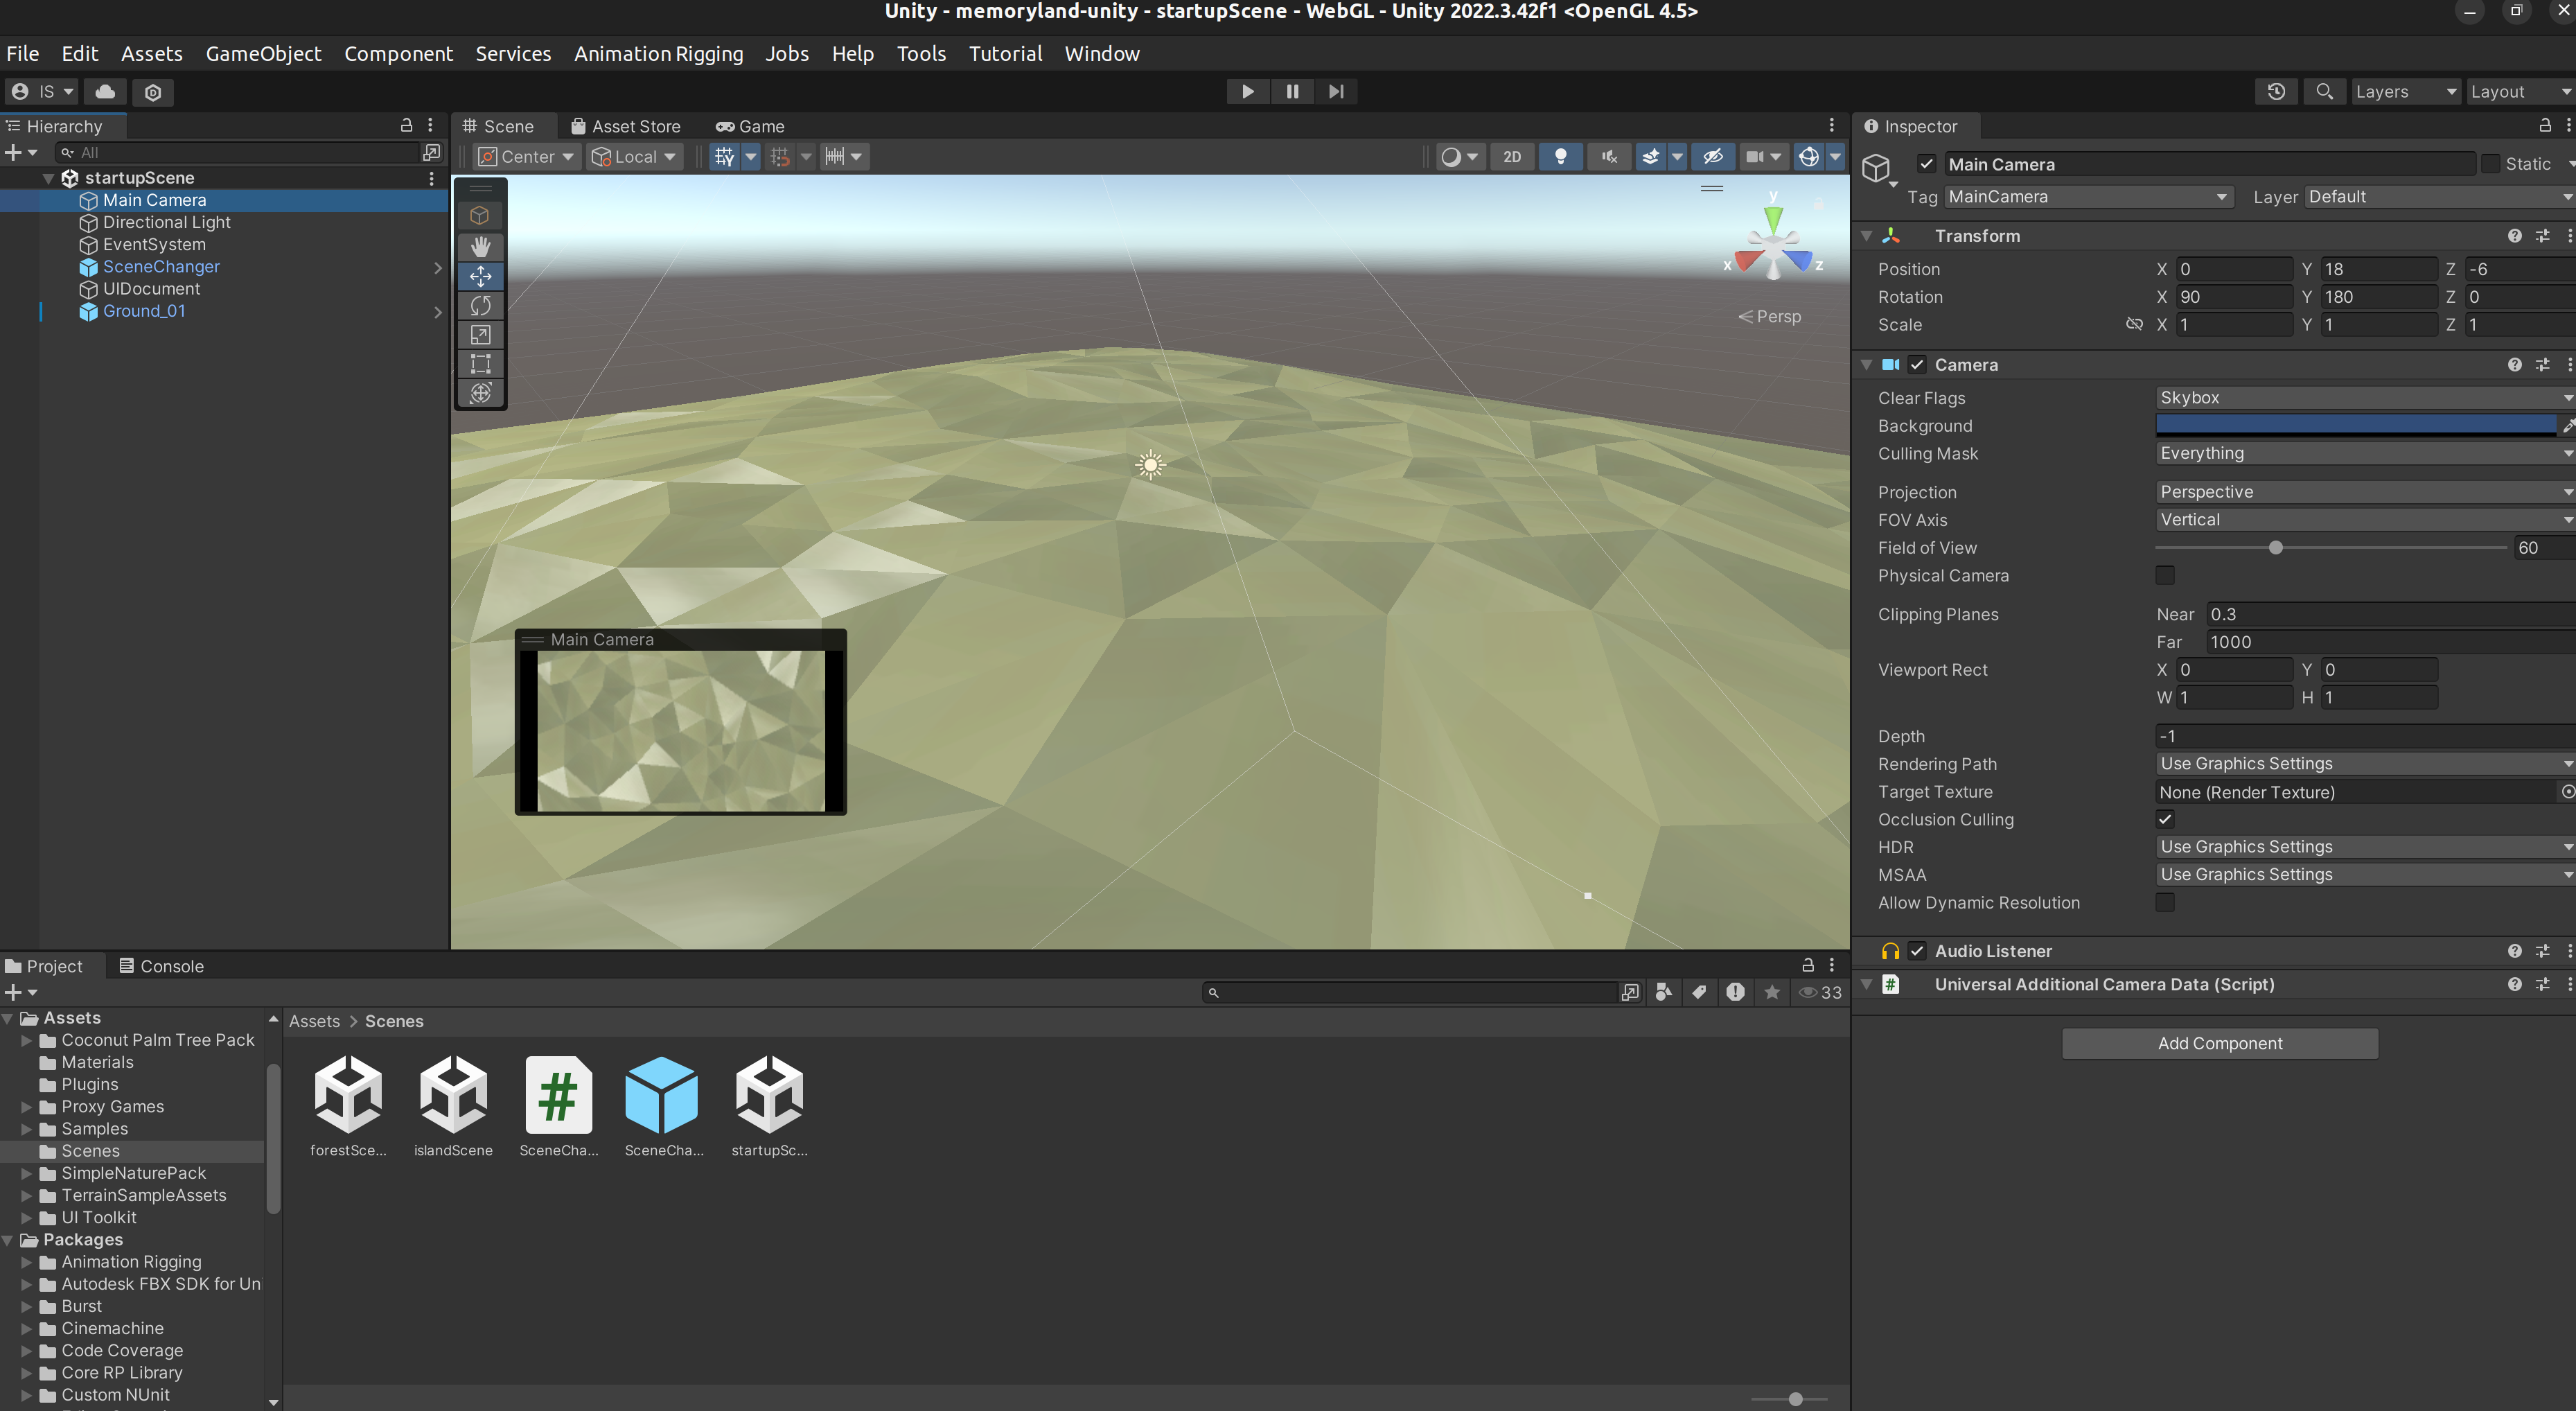
\includegraphics[scale=0.5]{pics/unity-ide.png}
    \caption{Entwicklung in Unity: Die Unity IDE}
    \label{fig:unity-ide}
\end{figure}


Der Entschluss diese Technologie zu verwenden fiel vor allem, weil diese Technologie bereits frühzeitig in unserem Lehrplan enthalten ist und damit umfangreiche Kenntnisse vorhanden waren. Der andere, wesentliche Grund liegt in der Erweiterbarkeit der Umgebung die man in Unity schafft. Die Entwicklungsumgebung ist dergestalt, dass man von Beginn an mit mehreren Scenen im Entwurf gearbeitet hat. Jede Szene (Scene) in Unity spiegelt dabei einen Memorylandtype\footnote{siehe dazu vor allem Abschnitt \ref{}}



\subsection{Visual Studio}


\section{Einrichtung von Unity}

% noch genauer Query Params erklären

\section{Erstellung von neuen Memoryland-Typen}

\section{Einfügen von Images}



